\chapter{The Sun, the Photographs and the Labels}\label{ch:data}

\section{Introduction}\label{sec:data-intro}
\epigraph{It is a capital mistake to theorize before one has data.}{Sherlock Holmes, in Arthur
Conan Doyle, \emph{A Scandal in Bohemia} \citeyearpar{doyle1891}}

Before we build any model, we need to understand what the photographs show and how their labels
were made. In this chapter we review just enough solar physics to interpret the images
(Section~\ref{sec:data-sun}), describe the telescopes that took them
(Section~\ref{sec:data-gong}) and the annotations that label them
(Section~\ref{sec:data-magfilo}), summarise the rules of the competition
(Section~\ref{sec:data-rules}), and finally draw some conclusions for modelling
(Section~\ref{sec:data-implications}). Several of the facts collected here, such as the width of
a typical filament and the number of annotators per photograph, will determine important design
choices in later chapters.

\section{Enough solar physics to read the pictures}\label{sec:data-sun}
One does not need to be a solar physicist to work on this problem, but a few facts explain what
the photographs show and why the labels look the way they do.

The visible surface of the Sun, the \keyterm{photosphere}, is covered by a thin and hotter layer
called the \keyterm{chromosphere}~\citep{stix2002}. Hydrogen in the chromosphere absorbs and emits light at a
wavelength of 656.3~nm, the red \keyterm{\Ha{} line}. A filter that passes only a narrow band
around this wavelength blocks most of the light from the photosphere, so an \Ha{} image shows the
chromosphere instead. In this light the disk is covered by a mottled pattern of darker and
brighter cells called the \keyterm{chromospheric network}, with bright patches called
\keyterm{plage} around the active regions where sunspots form.

A \keyterm{filament} is a cloud of plasma that is cooler and denser than its surroundings, held
above the surface by the Sun's magnetic field~\citep{mackay2010}. It lies along a
\keyterm{polarity inversion line}, a curve on the surface across which the vertical component of
the magnetic field changes sign. Seen against the bright disk, the cool plasma absorbs \Ha{}
light, so the filament appears as a dark thread. Seen at the edge of the disk against the dark
sky, the same structure glows, and it is then called a \keyterm{prominence}~\citep{parenti2014}. A
filament has a central \keyterm{spine} and often thin side branches called \keyterm{barbs}.
Whether the barbs bear to the left or to the right encodes the filament's \keyterm{chirality}, a
property of its magnetic field~\citep{martin1998}. Filaments persist for days to weeks, drift
across the disk as the Sun rotates (about once every 27 days), and sometimes erupt, which is why
space-weather forecasting is interested in them~\citep{webb2012,magfilo}.

Three consequences of this physics matter for modelling. First, filaments are dark, but darkness
does not identify them, because the chromospheric network covers the same range of intensities.
This is why simple thresholding of the image does not work, as we show in
Section~\ref{sec:recall-physics}. Second, filaments fade gradually into their surroundings. There
is no sharp edge, so the position of a filament's boundary is a judgement made by the annotator;
Figure~\ref{fig:post-profile} in Chapter~\ref{ch:post} plots the intensity across a real
filament. Third, filaments persist. Photographs taken a day apart show the same filaments, and
this affects how we must split the data into training and validation sets
(Section~\ref{sec:val-time}).

Finally, the disk is darker towards its edge. This \keyterm{limb darkening}~\citep{stix2002} occurs because near
the limb our line of sight passes through the solar atmosphere at a grazing angle. It dims both
the filaments and their surroundings there, so a filament near the limb looks different from one
near the centre of the disk.

\section{The GONG network and its photographs}\label{sec:data-gong}
The photographs come from the \keyterm{Global Oscillation Network Group} (GONG), a set of six
identical telescopes placed around the world so that at least one of them can observe the Sun at
any time~\citep{gong,jain2026gong}.\footnote{GONG is operated by the US National Solar Observatory.
It was built to study oscillations of the Sun's surface, and \Ha{} imaging was added to its
stations later to support the monitoring of space weather~\citep{hill2018}.} The stations are at
Big Bear in California (station code Bh), Mauna Loa in
Hawaii (Mh), Learmonth in Australia (Lh), Udaipur in India (Uh), El Teide in the Canary Islands
(Th) and Cerro Tololo in Chile (Ch). Each station records full-disk \Ha{} images. For the
competition, the images were converted from the astronomical FITS format~\citep{pence2010} into 8-bit grey JPEG
files of $2048\times2048$ pixels. The file name records the time of capture and the station; for
example, \file{20140609195854Bh.jpeg} was taken at Big Bear on 9 June 2014 at 19:58:54.

\begin{figure}[t]
\centering
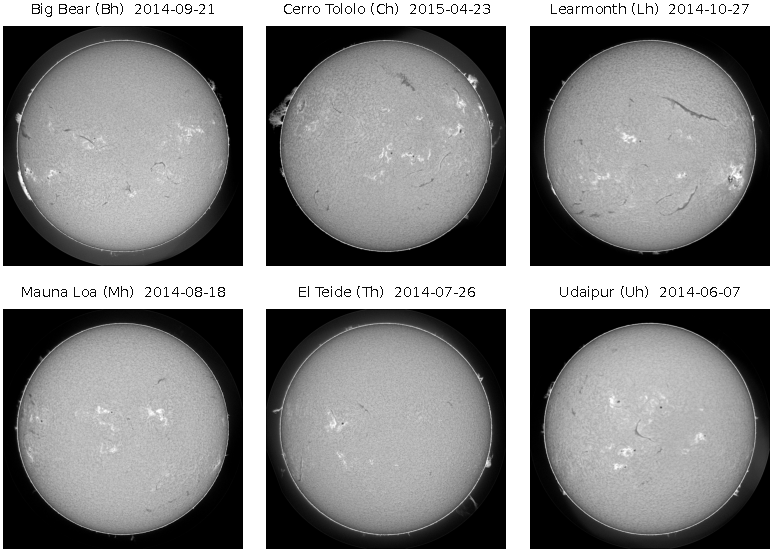
\includegraphics[width=\textwidth]{figures/fig_stations.pdf}
\caption{One training photograph from each GONG station, with the display contrast stretched. The
stations differ in atmospheric seeing, in contrast and in the brightness of the limb. Bright
prominences are visible outside the limb in several of the frames.
\generatedby{book/make\_book\_figures.py:fig\_stations}}
\label{fig:data-stations}
\end{figure}

Figure~\ref{fig:data-stations} shows one photograph from each station. Although the instruments
are identical, the atmosphere above them is not, so the sharpness and contrast of the images vary
from frame to frame, and a model must cope with this variation. On the other hand, the Sun fills
the same circle in every frame, surrounded by black sky, so a model can easily learn where the
disk is.

The training photographs span the years 2011 to 2022, and the test photographs are drawn from the
same years and stations in almost the same proportions (Figure~\ref{fig:data-years}). The dip in
2018--2020 corresponds to the solar minimum, when there are fewer active regions and therefore
fewer filaments to label. We checked this agreement early in the project. A difference between
the training and test distributions, often called \keyterm{covariate shift}, is one of the usual
explanations when validation scores fail to carry over to a leaderboard
(Section~\ref{sec:val-transfer}), and the figure shows that it cannot explain our results.

\begin{figure}[t]
\centering
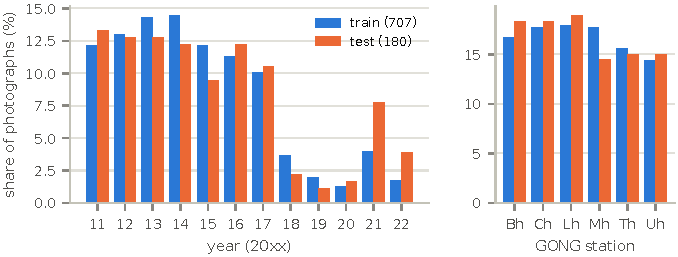
\includegraphics[width=\textwidth]{figures/fig_years.pdf}
\caption{Share of photographs by year (left) and by GONG station (right), for the \AllPhotos{}
training photographs and the \TestPhotos{} test photographs.
\generatedby{book/make\_book\_figures.py:fig\_years}}
\label{fig:data-years}
\end{figure}

\section{The MAGFiLO annotations}\label{sec:data-magfilo}
The labels come from MAGFiLO, the Manually Annotated GONG Filaments in \Ha{} Observations
dataset~\citep{magfilo}, which is released under the Creative Commons BY-NC-ND 4.0 licence. The
competition supplies a subset of it as a single JSON file in the format of the COCO
dataset~\citep{coco}. The file contains three lists that matter to us.
\begin{description}[style=unboxed,leftmargin=1em,itemsep=2pt,font=\normalfont\bfseries]
\item[\texttt{images}] One entry per \emph{annotation record}. Its \texttt{id} joins an
annotator's batch number to the name of the photograph, as in \texttt{040301-20140609195854Bh},
and its \texttt{file\_name} names the photograph.
\item[\texttt{annotations}] One entry per filament, containing a \texttt{segmentation} polygon,
a \texttt{spine} polyline along the filament's centre, a \texttt{bbox}, an \texttt{area}, a
\texttt{category\_id}, and the \texttt{image\_id} of the record the filament belongs to.
\item[\texttt{categories}] Four labels, \emph{Left}, \emph{Right}, \emph{Unidentifiable} and
\emph{Ambiguous}, which record the filament's chirality. The competition ignores them and treats
every filament simply as a filament.
\end{description}

Listing~\ref{lst:data-load} reads the file and groups the records by photograph. Every data
loader in the repository has essentially this shape.

\begin{lstlisting}[caption={Grouping annotation records by photograph. Adapted from \file{shared/data\_split.py:load\_records}.},label=lst:data-load]
import json
from collections import defaultdict

coco = json.load(open("data/MAGFiLO_1.0_Annotations_kaggle2026_train.json"))
records_by_photo = defaultdict(list)      # file_name -> [record id, ...]
for image in coco["images"]:
    records_by_photo[image["file_name"]].append(image["id"])
filaments = defaultdict(list)             # record id -> [annotation, ...]
for annotation in coco["annotations"]:
    filaments[annotation["image_id"]].append(annotation)

print(len(coco["images"]), "records of", len(records_by_photo), "photographs")
print(len(coco["annotations"]), "filaments")
\end{lstlisting}

The listing prints \AllRecords{} records of \AllPhotos{} photographs and \AllFilaments{}
filaments. Of the photographs, \OnceAnnotated{} were labelled once, \TwiceAnnotated{} twice and
\ThriceAnnotated{} three times, by independent annotators who did not see each other's work.
Figure~\ref{fig:intro-annotators} in Chapter~\ref{ch:intro} showed how different their results
can be.

\subsection{Records and photographs}\label{sec:data-records}
Since some photographs have several records, we must decide whether the unit of our data is the
photograph or the record. The metric answers this question for us. As we will see in
Section~\ref{sec:metric-pooling}, each record is scored separately, against the one annotator who
made it. A model that is scored against three annotators on the same photograph is therefore
asked three slightly different questions, one per annotator. For this reason the final model
treats every record as a separate training sample (Section~\ref{sec:train-sampling}): a
photograph with three records is seen three times, each time with one annotator's masks.

Getting this unit wrong has real consequences. In Chapter~\ref{ch:recall} we describe a
classifier that we trained to decide whether a candidate mask was a real filament. We labelled a
candidate as positive if \emph{any} annotator of the photograph had drawn a filament at that
location. The classifier learned this task well, with a precision of 72\% on its own validation
data, but when we used it to choose which candidates to submit, only 17\% of its choices matched
the annotator of the record being scored (Section~\ref{sec:recall-verifiers}). The classifier had
answered the question ``would somebody draw this?'', whereas the metric asks ``did this particular
person draw it?''.

\subsection{How big are filaments?}\label{sec:data-sizes}
Figure~\ref{fig:data-stats} summarises the sizes of the annotated filaments. The median bounding
box is \LongPfifty{} pixels on its long side; 90\% of filaments are shorter than \LongPninety{}
pixels and 99\% are shorter than \LongPninetynine{}, and the longest is \LongMax{} pixels long.
The median area is \AreaMedian{} pixels. A record contains \MeanPerRecord{} filaments on average
and at most \MaxPerRecord{}, and no record is empty.

\begin{figure}[t]
\centering
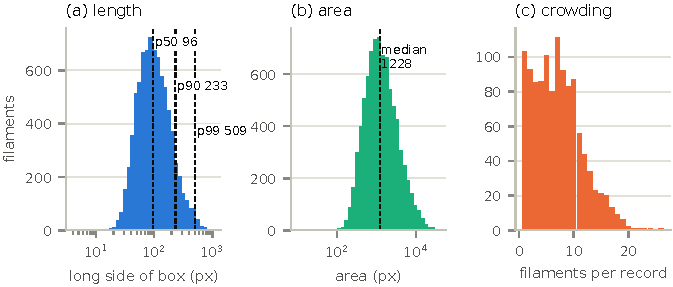
\includegraphics[width=\textwidth]{figures/fig_filament_stats.pdf}
\caption{Filament sizes and crowding over all \AllFilaments{} training annotations. (a) The long
side of the bounding box, with the 50th, 90th and 99th percentiles marked. (b) The area. (c) The
number of filaments per annotation record.
\generatedby{book/make\_book\_figures.py:fig\_filament\_stats}}
\label{fig:data-stats}
\end{figure}

These numbers will turn into design decisions later. Since 99\% of filaments are shorter than
about 510 pixels, a $1024\times1024$ crop centred on a filament almost always contains it whole,
which is why the final model trains on crops of that size (Section~\ref{sec:train-sampling}).
Since a record contains at most \MaxPerRecord{} filaments, a model that proposes 100 candidate
objects per image always has enough of them (Section~\ref{sec:tr-m2f}). And since filament bodies
are only a few pixels wide, resolution matters a great deal: a body four pixels wide in the
native $2048\times2048$ image is only one pixel wide after the image is shrunk to
$512\times512$.

\subsection{Spines}\label{sec:data-spines}
Every annotation also contains a spine, a polyline traced along the filament's axis. We used the
spines in two experiments. The first (exp004) planned to use predicted spines to decide which
pixels belong to which filament, and an ablation led us to drop the idea before any model was
trained (Section~\ref{sec:paradigms-fragments}). The second (exp085) trained a semantic model with
an additional output that predicts the spine (Section~\ref{sec:recall-semantic}). Neither became
part of the final pipeline. Nevertheless, the spine is the most direct description of a
filament's shape, and it remains a natural input for future work.

\section{The competition's rules}\label{sec:data-rules}
The rules of the competition shape the work as much as the data do.
\begin{itemize}[leftmargin=*,itemsep=2pt]
\item \textbf{Submission format.} A submission contains one CSV row per predicted filament: an
identifier of the form \texttt{<photograph>\_<k>}, and the mask as a COCO run-length encoding
without its size field, since the size is always $2048\times2048$ (Chapter~\ref{ch:masks}).
\item \textbf{No overlaps.} The masks predicted for one photograph must be disjoint. The scorer
rejects a file in which two masks share a pixel.
\item \textbf{The leaderboard.} The public leaderboard scores about half of the test photographs
and displays the score to two decimal places. The final ranking uses the other half.
\item \textbf{The rubric.} The final judgement is 70\% quantitative and 30\% qualitative. The
quantitative part uses PQ together with the distributions of the Dice coefficient, of IoU and of
the one-to-many relations between predicted and annotated filaments. The qualitative part is based
on a four-page technical report and on the code. The competition's host has also said that the
judges will look at individual predictions and at the logic of the algorithm, and not only at
the score.
\end{itemize}

\subsection{A replaced evaluator and a data leak}\label{sec:data-history}
Two episodes in the competition's history explain some odd features of its leaderboard. Before
August 2026 the competition was scored with a metric based on the Dice coefficient, and this
metric could be exploited: a public notebook showed that submitting empty masks for five of the
180 test images produced a perfect score of 1.00. The organisers replaced the metric with
Panoptic Quality and rescored all submissions. Some very high scores that remain on the
leaderboard still come from methods that, according to the host, can be distinguished from
legitimate work.

The second episode is a leak. The full MAGFiLO dataset is public, and it contains the
competition's test photographs together with their annotations. Training on it would mean
training on the answers, so we never use it. The release is also smaller than it first appears.
The MAGFiLO paper reports 1,593 observations, but this number counts annotation passes; the
release contains 958 distinct photographs, of which the competition already uses 887.

\section{What the data imply for modelling}\label{sec:data-implications}
We end the chapter by collecting the facts above into five implications, each of which we will
meet again.
\begin{enumerate}[leftmargin=*,itemsep=2pt]
\item Resolution matters. Filaments are a few pixels wide, and shrinking the image destroys them
(Sections~\ref{sec:yolo-resolution} and~\ref{sec:train-resolution}).
\item Labels belong to records. We should train, and score, one annotator at a time
(Section~\ref{sec:data-records}).
\item Labels disagree. No model can match every annotator perfectly, so a perfect score is not a
useful reference point (Section~\ref{sec:metric-agreement}).
\item Photographs are not independent. The same filament appears in photographs taken days apart,
so a random split of the photographs leaks information from training to validation
(Section~\ref{sec:val-time}).
\item Position matters. Limb darkening and foreshortening make a filament near the edge of the disk
look different from one near its centre.
\end{enumerate}

\section*{Exercises}
\begin{exercise}{Decoding file names}
Write a function that turns \file{20110914063134Lh.jpeg} into a timestamp and a station name. Use
it to count the training photographs per station, and compare your counts with
Figure~\ref{fig:data-years}.
\end{exercise}

\begin{exercise}{Long filaments}
Using the \texttt{bbox} field, compute the fraction of filaments whose long side exceeds 512
pixels. Relate your answer to the crop size used in Chapter~\ref{ch:training}.
\end{exercise}

\begin{exercise}{Spine and polygon}
Choose one annotation, draw its polygon and its spine on the same axes, and compute the length of
the spine. Is the spine always inside the polygon?
\end{exercise}

\begin{exercise}{Chirality}
Count how often each of the four \texttt{category\_id} values occurs. Then, for photographs with
more than one annotator, estimate how often two annotators give the same category to a filament
that both of them drew. What does your answer suggest about using the categories as a training
signal?
\end{exercise}
